\chapter{Introduction}
This is the introduction of this \LaTeX\,template for master's thesis at TU Delft. Please use XeLaTeX as the compiler in settings. As you can see from the file tree, the general structure of this template includes:
\begin{itemize}
    \item \textit{Premeables}: \texttt{commands.tex} for self-defined commands, \texttt{layout.tex} of this template, and \texttt{packages.tex} for necessary pakages...
    \item \texttt{Chapter x.tex}: content of each chapter...
    \item \texttt{figures.tex}: all figures for this thesis
    \item \texttt{layout.tex} for the main body of this template
\end{itemize}
In the following sections, some coding examples are included for the \textit{Formulaes, Figures Tables, and inline citations}used in this template :)
\clearpage
\section{Formulae}
The motion of an isotropic, linear elastic soil layer is governed by Navier--Cauchy equation:
\begin{align}
\mu_{\mathrm{s}}\nabla^2\mathbf{u}_{\mathrm{s}}+\left(\lambda_{\mathrm{s}}+\mu_{\mathrm{s}}\right)\nabla\nabla\cdot\mathbf{u}_{\mathrm{s}} - \rho_{\mathrm{s}}{\ddot{\mathbf{u}}}_{\mathrm{s}}=0,
\label{eq: Navier-Cauchy Equation}
\end{align}
\section{Figures}
\subsection{Tikz figure}
Figures below are made by tikz module in \LaTeX:
\begin{figure}[h!]
\begin{subfigure}[t]{0.48\textwidth}
\caption{Fluid waveguide: single layer}
\label{fig: roots fluid waveguide}
    \centering
    \scalebox{0.8}{
   \begin{tikzpicture}
    % draw layers
        % \fill[pattern=north east lines, pattern color=gray!40] (0,0) rectangle (-3.1,-3.1);
    % draw axis
        \draw[axis] (-3.0,0) -- (3.0,0) node[right] {\small $\mathrm{Re}(k_r)$};
        \draw[axis] (0,-2.1) -- (0,2.1) node[above] {\small $\mathrm{Im}(k_r)$};
        % \draw[line width=2.0pt] (0,0) -- (0,-3.8);
        % \draw[line width=2.0pt] (0,0) -- (2,0);
        \filldraw (2,0) circle (2pt) node[above, yshift = 0.3mm] {$k_{\mathrm{f}}$};
        \filldraw (-2,0) circle (2pt) node[above, yshift = 0.3mm] {$k_{\mathrm{f}}$};
        \filldraw[fill=white, draw=black](-0.5,0) circle (1.5pt);
       \filldraw[fill=white, draw=black] (-0.25,0) circle (1.5pt);
        \filldraw[fill=white, draw=black] (-0.75,0) circle (1.5pt);
        \filldraw[fill=white, draw=black] (-1.5,0) circle (1.5pt);
        \filldraw[fill=white, draw=black] (-1.75,0) circle (1.5pt);
       \filldraw[fill=white, draw=black] (-1,0) circle (1.5pt);
        \filldraw[fill=white, draw=black] (-1.25,0) circle (1.5pt);

        \filldraw (0.5,0) circle (1.5pt);
        \filldraw (0.25,0) circle (1.5pt);
        \filldraw (0.75,0) circle (1.5pt);
        \filldraw (1.5,0) circle (1.5pt);
        \filldraw (1.75,0) circle (1.5pt);
        \filldraw (1,0) circle (1.5pt);
        \filldraw (1.25,0) circle (1.5pt);

        \filldraw (0,-0.5) circle (1.5pt);
        \filldraw (0,-0.25) circle (1.5pt);
        \filldraw (0,-0.75) circle (1.5pt);
        \filldraw (0,-1.5) circle (1.5pt);
        \filldraw (0,-1.75) circle (1.5pt);
        \filldraw (0,-1) circle (1.5pt);
        \filldraw (0,-1.25) circle (1.5pt);

        \filldraw[fill=white, draw=black] (0,0.5) circle (1.5pt);
        \filldraw[fill=white, draw=black] (0,0.25) circle (1.5pt);
        \filldraw[fill=white, draw=black](0,0.75) circle (1.5pt);
        \filldraw[fill=white, draw=black] (0,1.5) circle (1.5pt);
        \filldraw[fill=white, draw=black] (0,1.75) circle (1.5pt);
        \filldraw[fill=white, draw=black] (0,1) circle (1.5pt);
        \filldraw[fill=white, draw=black] (0,1.25) circle (1.5pt);
    \end{tikzpicture}}
    \end{subfigure}
\begin{subfigure}[t]{0.48\textwidth}
\centering
    \caption{Lossless single elastic waveguide}
    \label{fig: roots elastic waveguide_lossy}
    \scalebox{0.8}{
      \begin{tikzpicture}
        % draw layers
            % \fill[pattern=north east lines, pattern color=gray!40] (0,0) rectangle (-3.1,-3.1);
        % draw axis
            \draw[axis] (-3.0,0) -- (3.0,0) node[right] {\small $\symrm{Re}(k_r)$};
            \draw[axis] (0,-2.1) -- (0,2.1) node[above] {\small $\symrm{Im}(k_r)$};
            % \node at (1.5,-2.9) {$\mathcal{C}^{\infty}$};
            % \node at (-1.2,-1.2) {\small $S_1$};
            % \node at (0.3,-1.2) {\small $\Theta_1$};
            % \node at (1.2,-1.4) {\small $\Theta_2$};
            % \draw[line width=2.0pt] (0,0) -- (0,-3.8);
            % \draw[line width=2.0pt] (0,0) -- (2,0);
            % \filldraw (2.5,0) circle (2pt) node[above, yshift = 0.3mm] {\small $k_{\mathrm{T,2}}$};
            \filldraw (2.4,0) circle (1.5pt);
            \filldraw (1.6,0) circle (1.5pt);
            \filldraw (1.8,0) circle (1.5pt);
            \filldraw (0.6,0) circle (1.5pt);
            \filldraw (0.8,0) circle (1.5pt);
            \filldraw[fill=white, draw=black](-2.4,0)circle (1.5pt);
            \filldraw[fill=white, draw=black](-1.6,0)circle (1.5pt);
            \filldraw[fill=white, draw=black](-1.8,0)circle (1.5pt);
            \filldraw[fill=white, draw=black](-0.6,0)circle (1.5pt);
            \filldraw[fill=white, draw=black](-0.8,0)circle (1.5pt);
            % \filldraw (-2.5,0) circle (2pt) node[above, yshift = 0.3mm] {\small $-k_{\mathrm{T,2}}$};
            \filldraw (1.2, 0) circle (2pt) node[above,yshift=0.3mm] {\small $k_{\symrm{L}}$};
            \filldraw (2, 0) circle (2pt) node[above,yshift=0.3mm] {\small $k_{\symrm{T}}$}; 
            \filldraw (-1.2, 0) circle (2pt) node[above,yshift=0.3mm] {\small $-k_{\symrm{L}}$};
            \filldraw (-2, 0) circle (2pt) node[above,yshift=0.3mm] {\small $-k_{\symrm{T}}$}; 
           \foreach \x in {0,0.2,...,0.8} {
            \draw[fill=black, draw=black] (\x, {-2.5*\x^2-0.5}) circle (1.5pt);
            }
              \foreach \x in {0,0.2,...,0.8} {
           \draw[fill=white, draw=black] (-\x, {2.5*\x^2+0.5}) circle (1.5pt);
        }
        \foreach \x in {0.2,0.4,...,0.8} {
              \draw[fill=white, draw=black](\x, {2.5*\x^2+0.5}) circle (1.5pt);
        }
        \foreach \x in {0.2,0.4,...,0.8} {
            \draw[fill=black, draw=black](-\x, {-2.5*\x^2-0.5}) circle (1.5pt);
        }
        \foreach \x in {0.1,0.3} {
            \draw[fill=black, draw=black]  (0, {-\x}) circle(1.5pt);
        }
        \foreach \x in {0.1,0.3} {
            \draw[fill=white, draw=black]  (0, {\x}) circle(1.5pt);
        }
        \end{tikzpicture}}
\end{subfigure}
\hfill
\centering
\begin{subfigure}[t]{0.48\textwidth}
\centering
    \caption{Lossy single elastic waveguide}
    \label{fig: roots elastic waveguide}
    \scalebox{0.8}{
      \begin{tikzpicture}
        % draw axis
        \draw[axis] (-3.0,0) -- (3.0,0) node[right] {\small $\symrm{Re}(k_r)$};
        \draw[axis] (0,-2.1) -- (0,2.1) node[above] {\small $\symrm{Im}(k_r)$};

        % k_L and k_T in the 4th quadrant
        \coordinate (kL) at (1.0, -0.2);
        \coordinate (kT) at (2.0, -0.3);
        \filldraw (kL) circle (1.8pt) node[right] {\small $k_{\symrm{L}}$};
        \filldraw (kT) circle (1.8pt) node[right] {\small $k_{\symrm{T}}$};

        % k_L branch - gently curving down-right
        \foreach \i in {2,...,10} {
            \pgfmathsetmacro{\x}{0.1*\i}
            \pgfmathsetmacro{\y}{-0.2/(0.1*\i)}
            \filldraw (\x,\y) circle (1pt);
        }

        % k_T branch - similar curve
        \foreach \i in {2,...,10} {
            \pgfmathsetmacro{\x}{0.2*\i}
            \pgfmathsetmacro{\y}{-0.6/(0.2*\i)}
            \filldraw (\x,\y) circle (1pt);
        }
    \end{tikzpicture}
    }
\end{subfigure}
\caption{Indicative positions of eigenvalues for different bounded layered media}
\end{figure}
\clearpage
\subsection{Normal figure}
\begin{figure}[h]
  \centering
  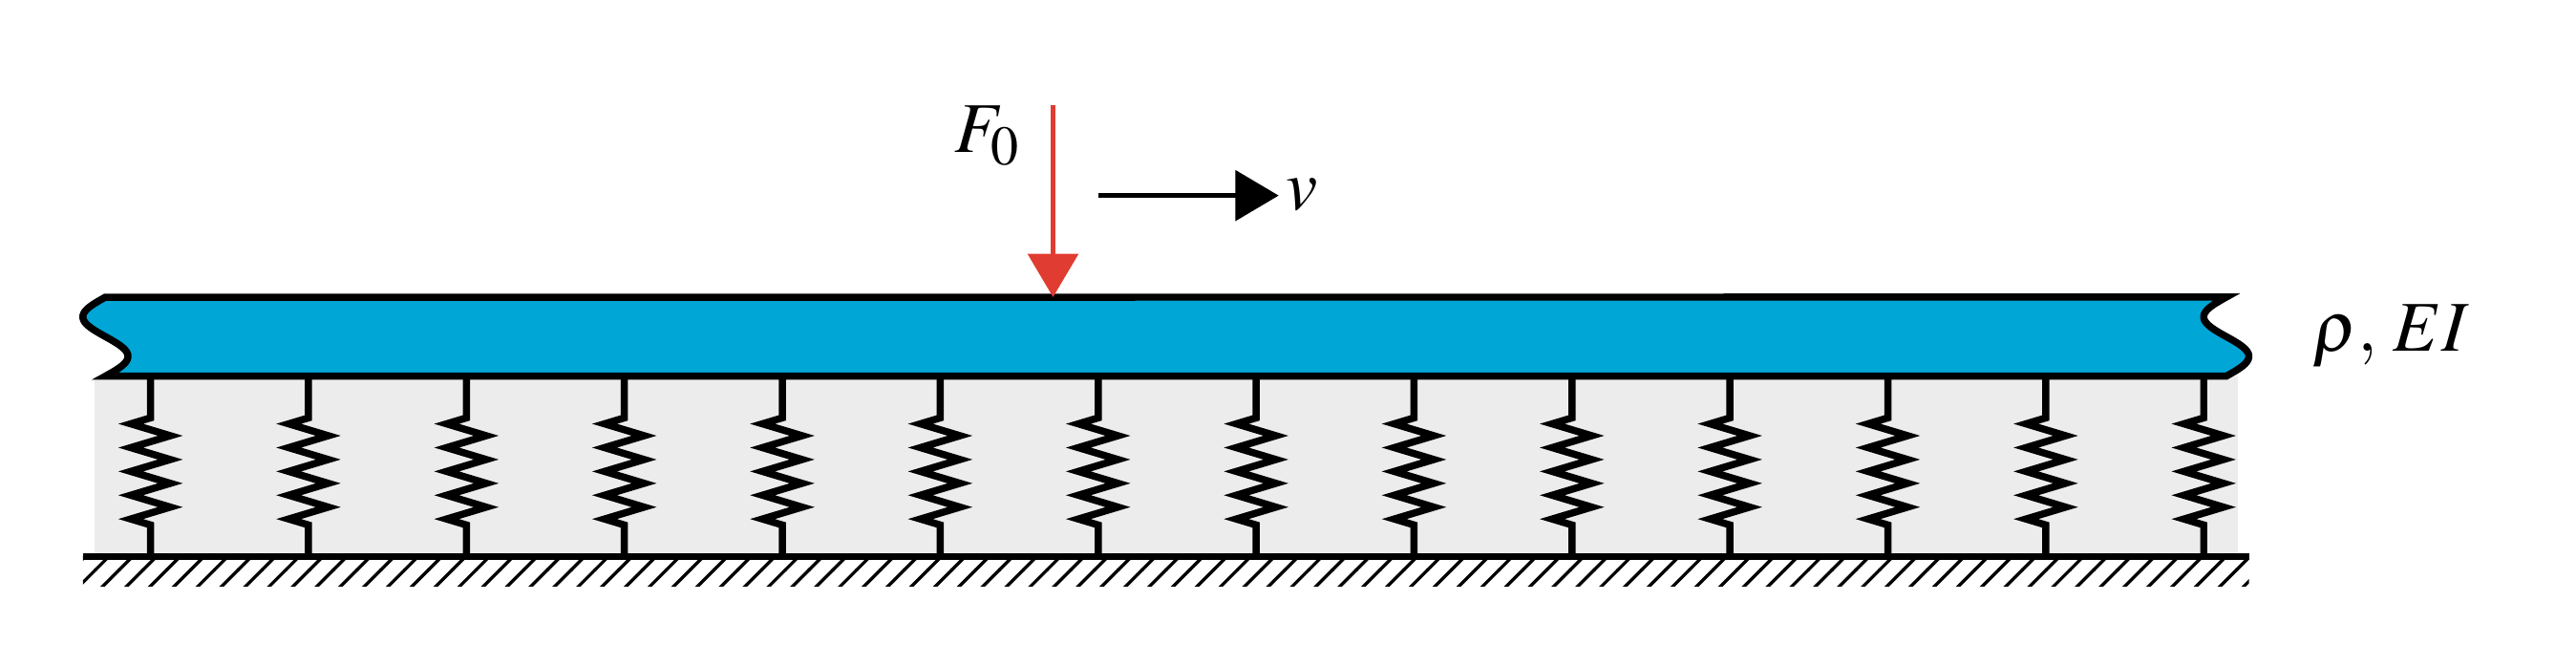
\includegraphics[width=0.9\textwidth]{figures/beam_load.png}   % or \includegraphics if you prefer the PDF
  \caption{Moving load on a finite Euler-Bernoulli beam}
  \label{fig:c1_beam_load}
\end{figure}
\subsection{Flow chart}
\begin{figure}[h!]
\scalebox{0.7}{
\begin{tikzpicture}[node distance=1.3cm]
            % \draw[rounded corners=10pt, fill=gray!10, dashed, thick] (-2,0.8) rectangle (9.3,-11);
            % Nodes
            \draw[rounded corners=10pt,fill=gray!10, dashed, thick] (7,4.5) rectangle (14,3);
            \node (case 1) [process] {{Waveguide-PML}};
            \node (fluid density) [input, right of = case 1, xshift = 7.5 cm, yshift = 2.0cm] {{Material properties}};
            \node (layer thickness) [input, right of = case 1, xshift = 7.5 cm, yshift = 0.4cm] {{Layer thickness}};
            \node (fluid domain) [process, right of = case 1, xshift = 3.5 cm, yshift = 1.2 cm] {{Physcial domain}};
            \node (PML domain) [process, right of = case 1, xshift = 3.5 cm, yshift = -1.2 cm] {{PML domain}};
            \node (PML thickness) [input, right of = case 1, xshift = 7.5 cm, yshift = -0.4cm] {{PML thickness} $H_{\symrm{PML}}$};
            % \node (scaling) [input, right of = case 1, xshift = 7.5 cm, yshift = -1.2cm] {Scaling function $\alpha_s(z)$};
            \node (attenuation) [input, right of = case 1, xshift = 7.5 cm, yshift = -2.0cm] {{Complex stret. function} $\beta(z)$};
            % \node (alpha0) [input,right of = case 1, xshift = 11 cm, yshift = -0.4cm] {tuning scalar $\alpha_0$};
            \node (m) [input,right of = case 1, xshift = 11 cm, yshift = -1.2cm] {{polynomial order} $m_{\symrm{PML}}$};
            \node (beta0) [input, right of = case 1, xshift = 11 cm, yshift = -2.0cm] {{tuning scalar} $\beta_0$};
            
            \node (analytical 1) [process, below of = case 1, yshift = -0.4cm] {{Dispersion relations}};
            \node (root 1) [process, below of = analytical 1, yshift = -0.4cm] {{Eigen values}};
            \node (eigen functions) [process, right of = root 1, xshift = 3.5cm] {{Eigen vectors}};
            \node (freq) [input, right of = case 1,xshift = 7.5cm, yshift = -2.8cm] {{Frequency} $\omega$};
            % \node (kr) [output, below of = freq, yshift = -1.0cm] {Radial wavenumber $k_r$};
            % \node (MC1) [process, below of = root 1, yshift = -0.4cm] {Classification};
            \node (DC) [process, right of = root 1, xshift = 7.5 cm, yshift = -0.5cm] {{Dispersion curves}};
            % \node (MS) [process, below of = DC, yshift = -0.4cm] {Modal Shapes};
            % \node (ortho) [process, below of = MS,yshift = -0.4cm] {Orthogonality Check};
            % \node (PML) [output, right of = MC1, xshift = 3.5cm, yshift = 0.5cm] {PML Mode};
            % \node (Guided 1) [output, right of = MC1, xshift = 3.5cm, yshift = -0.5cm] {Guided Mode};
            \node (cg) [output, right of = DC,  xshift = 2cm, yshift = 0.4cm] {{Group velocity} $c_{\symrm{g}}$};
            \node (cp) [output, right of = DC,  xshift = 2cm, yshift = -0.4cm] {{Phase velocity} $c_{\symrm{ph}}$};
            \node (normalized mode) [output, below of = eigen functions, yshift = -2.0cm] {{Normalized modes}};
            \node (Orthogonality check) [process, right of = normalized mode, xshift = 2.5cm] {{Orthogonality}};
            \node (ana) [process, right of = Orthogonality check, xshift = 2.5cm] {{Anomalous dispersion?}};
            \node (label 1) [input, right of = fluid density, xshift = 2cm, yshift = 1.5cm] {{independent variables}};
            \node (integrationsize) [input, right of = Orthogonality check, xshift = 2.2cm, yshift = 1.2cm] {{Integration step} $\mathrm{d}z$};
            \node (label 2) [output, left of = label 1, xshift = -2cm,] {{dependent variables}};
            \node (label 3) [above of = label 2, yshift = -0.7cm, xshift = -0.8cm] {\footnotesize \textbf{{Labels}}};
            % \node (yes?) [check, right of = ortho, xshift = 2cm] {Ok?};
            
            % \node (ana) [process, right of = yes?, xshift = 2.5cm] {Check Anomalous Dispersion};
            
            \draw[arrow] (fluid density) -- ++(-2cm,0) |- (fluid domain.east);
            \draw[arrow] (layer thickness) -- ++(-2cm,0) |- (fluid domain.east);

            % \draw[arrow] (MC1.east) -- ++(+1.5cm,0) |- (PML.west);
            % \draw[arrow] (MC1.east) -- ++(+1.5cm,0) |- (Guided 1.west);
          

            % \draw[arrow] (m) -- (scaling.east);
            % \draw [arrow](alpha0) -- ++(-1.6cm,0cm) |- (scaling.east);
            \draw[arrow] (beta0) -- (attenuation.east);
            \draw[arrow](m.west) -- ++(-1.5,0)-| (attenuation.north);
            
            \draw[arrow] (PML thickness) -- ++(-2cm,0) |- (PML domain.east);
            % \draw[arrow] (scaling) -- (PML domain.east);
            \draw[arrow] (attenuation) -- ++(-2cm,0) |- (PML domain.east);
            \draw[arrow] (PML thickness) -- ++(-2cm,0) |- (PML domain.east);
            % \draw[arrow] (scaling) -- (PML domain.east);
            \draw[arrow] (attenuation) -- ++(-2cm,0) |- (PML domain.east);
            \draw[arrow] (freq) -- ++(-3cm,0) |- ([yshift = 0.1cm]analytical 1.east);
            \draw[arrow] ([yshift = -0.1cm] analytical 1.east) -- ++(1cm,0)node[anchor=west,yshift = -0.8cm]{\scriptsize}  |-([yshift = 0.1cm]eigen functions.west);

             % Arrows
             \draw[arrow] ([yshift=-0.1cm]integrationsize.west) -| (Orthogonality check.north);
        
            \draw[arrow] (PML domain.west)  -- ++(-1.2cm,0) |- (case 1.east) ;
            \draw[arrow]  (fluid domain.west)  -- ++(-0.985cm,0) |-(case 1.east);
            
            \draw [arrow]  (case 1.south) -- node[anchor=east]{\scriptsize {Formulation}} (analytical 1.north);
            \draw [arrow]  ([xshift = 0.3cm]root 1.north) --([xshift = 0.3cm]analytical 1.south);
            \draw [arrow]  ([xshift = -0.3cm]analytical 1.south) -- node[anchor=east]{\scriptsize {Root-Finding}} ([xshift = -0.3cm] root 1.north);
            \draw [arrow]  (root 1.south) |- ( DC.west);
            % \draw [arrow]  ([xshift = -1.2cm]kr.north) -- ++(-1.2cm,1.4cm)--(eigen functions.east);
            
            % \draw [arrow]  (root 1) -- node[anchor=east]{\scriptsize Residue Theorem } (MC1);
            \draw [arrow]  (freq.south) -- (DC.north);
            % \draw [arrow]   (kr.north) -- (DC.south);
            % \draw[arrow] (PML.east) -- ++(+1cm,0) |- (kr.west);
            % \draw[arrow] (Guided 1.east) -- ++(+0.845cm,0) |- (kr.west);
            \draw [arrow] (DC.east)  -- ++(+0.3cm,0) |- (cg.west);
            % \draw [arrow] (kr.east)  -- ++(+0.13cm,0) |- (cg.west);
             \draw [arrow] (DC.east)  -- ++(+0.3cm,0) |- (cp.west);
            % \draw [arrow] (kr.east)  -- ++(+0.13cm,0) |- (cp.west);
            \draw [arrow] ([yshift = -0.1cm]eigen functions.west)  --++(-1.5cm,0cm)--++(-0cm,-1.5cm) |- (normalized mode.west);
             \draw[arrow] (cp) -- ++(2.5cm,0) |- (ana.east);
             \draw[arrow] (cg) -- ++(2.5cm,0) |- (ana.east);
             \draw[arrow] (normalized mode.east) -- (Orthogonality check.west);
             \draw[arrow] ([yshift=0.1cm]Orthogonality check.east) -- ([yshift=0.1cm]ana.west);
            \draw[arrow] ([yshift=-0.1cm]ana.west) -- ([yshift=-0.1cm]Orthogonality check.east);
            % \draw [arrow]  (DC) -- (MS);
            % \draw [arrow]  (MS) -- (ortho);
            % \draw [arrow] (ortho) -- (yes?);
            % \draw [arrow] (yes?) -- node[anchor=north] {\scriptsize No} (ana);
            % \node at (7.4,-5.6) {\scriptsize Modal Tracking};
        \end{tikzpicture}}
    \caption{A Flow Chart of the theoretical framework of this thesis}
    \label{fig: ch2_framework}
\end{figure}
\clearpage
\section{Tables}
\begin{table}[h!]
    \centering
    \caption{Basic parameters used for numerical examples in Chapter 3}
    \label{table: fixed dimensions}
    \centering
    \renewcommand{\arraystretch}{1.0} % Adjust row spacing
    \setlength{\tabcolsep}{2.5pt} % Adjust column spacing
    \begin{tabular}{|l|llrl|l|llrl|}
        \hline
        \footnotesize{Elastic layer thickness}&\footnotesize{$H_\mathrm{EL}$}&& \footnotesize $10$ &\footnotesize m\\
        \footnotesize{Solid density upper layer}&\footnotesize$\rho_\mathrm{s}$ && \footnotesize $1700$&\footnotesize kg/m$^3$\\
        \footnotesize{Poisson's ratio}&\footnotesize$\nu$ && \footnotesize{$0.4$}&\footnotesize{-}\\
         \footnotesize Young's modulus &\footnotesize{$E_\mathrm{s}$} && \footnotesize $0.7$ &\footnotesize{MPa}\\
        \hline
    \end{tabular}
    \label{table: parameters elastic case}
    \end{table}
\section{Inline citations of figures and references}
For the single acoustic or elastic media with a rigid bottom, only discrete eigenvalues can be found, as shown indicatively in Figures~\ref{fig: roots fluid waveguide} and~\ref{fig: roots elastic waveguide}. Modes whose eigenvalues lie close to the real axis are referred to as trapped modes, as their energy remains confined within the waveguide due to repeated reflections at the rigid boundary~\cite{tsouvalas2014completeness}. In contrast, modes near the imaginary axis are known as evanescent modes, with energy localized near the source and rapidly decaying with range. 